\documentclass[12pt,twoside]{report}


\usepackage[utf8]{inputenc}
\usepackage[a4paper,width=150mm,top=25mm,bottom=25mm,bindingoffset=6mm]{geometry}
\usepackage{graphicx}
\graphicspath{ {images/} }

\usepackage[backend=bibtex,style=alphabetic,sorting=none]{biblatex}
\addbibresource{tex/references.bib}

\usepackage{fancyhdr}
\pagestyle{fancy}
\rhead{}

\usepackage{datetime}
\usepackage{hyperref}

\usepackage{amsmath}
\usepackage{amsfonts}
\usepackage{mathtools}


%% Definitions %%


\newcommand{\R}{\mathbb{R}}  % Pretty set of real numbers.
\newcommand{\me}{\mathrm{e}}  % Pretty Euler number.
\newcommand{\mi}{\mathrm{i}}  % Pretty imaginary unit.
\DeclarePairedDelimiter{\ceil}{\lceil}{\rceil}  % The ceiling function.


%% Document %%


\begin{document}


% Title page
\begin{titlepage}
	\begin{center}
		\vspace*{1cm}
		
		\LARGE
		Bachelor thesis
		
		\Huge
		\textbf{Online Event Detection from Text Data}
		
		\vspace{1.5cm}
		
		\Large
		\textbf{Tomáš Kala}

		\vspace{1cm}

		\Large
		Supervisor: doc. Ing. Jiří Kléma, PhD.
		
		\vfill

		\includegraphics[width=0.4\textwidth]{lion}
		
		\Large
		Department of Computer Science\\
		Faculty of Electrical Engineering\\
		Czech Technical University in Prague\\
		\monthname, \the\year
	\end{center}
\end{titlepage}


% Abstract
\thispagestyle{plain}

\begin{center}
	\Large
	\textbf{Abstract}
\end{center}

Event detection is a process of analysis of text documents aiming to uncover real events happening in the world. It is based on the assumption that words appearing in similar documents and time windows are likely to concern the same real-world event. Therefore, our method attempts to group together words with similar temporal and semantic characteristics while discarding noisy words, not contributing to anything of interest. This results in a concise event representation through a set of representative keywords. These are then used to query the document collection to retrieve the actual event-related documents. Finally, we extract short summaries from these documents and annotate the events in a human-readable fashion. The keyword retrieval phase of our method is based on an existing event detection system, which we modify by employing a word embedding model to measure semantic similarity. The method is evaluated on a collection of 2 million documents from Czech news over a 13 months period and compared to the original method, not depending on word embeddings.
\\
\\
\textbf{Keywords:} Document retrieval, event detection, multi-document summarization, word embedding.

\hfill

\begin{center}
	\Large
	\textbf{Abstrakt}
\end{center}

Detekce událostí je proces analýzy textových dokumentů za účelem odhalení událostí, které se během doby jejich vydání staly ve světě. Tento proces je založen na předpokladu, že sémanticky podobná slova se zvýšeným výskytem během stejného období se pravděpodobně vztahují ke stejné události. Námi zkoumaná metoda se tedy snaží shlukovat dohromady slova s podobnou časovou nebo sémantickou charakteristikou, a zároveň ignorovat slova nenesoucí žádnou informaci. To vede k jednoduché reprezentaci událostí pomocí skupin klíčových slov. Tato klíčová slova jsou následně použita k dotazu do zkoumané kolekce a získání dokumentů vztahujících se k jednotlivým událostem. Z těchto dokumentů jsou nakonec extrahována krátká shrnutí pro bohatší popis událostí. Fáze získávání klíčových slov je založena na existujícím postupu, který modifikujeme použitím modelu vnořování slov (word embedding) k měření sémantické podobnosti. Metoda je vyhodnocena na kolekci 2 milionů dokumentů z českých novinových serverů vydané za období 13 měsíců, a porovnána s původním postupem nevyžadujícím vnořování slov.
\\
\\
\textbf{Klíčová slova:} Získávání dokumentů, detekce událostí, sumarizace více dokumentů, word embedding.


% Declaration
\chapter*{Declaration}
This is my declaration.


% Acknowledgements
\chapter*{Acknowledgements}
These are my acknowledgements.


% Table of contents
\tableofcontents
\listoffigures


% Chapters
\chapter*{Introduction}
\addcontentsline{toc}{chapter}{Introduction}
As the number of news articles published each day grows, it becomes impossible to manually examine them all to learn about events happening in the world. The field of Event Detection arose as a subfield of Information Retrieval \citep{information-retrieval-2, information-retrieval} and Topic Detection and Tracking \citep{tdt, tdt-2} with a goal to aid the users by automatically discovering important events in document collections.

More precisely, given a stream of text documents published over a certain time period, the task is to analyze them and output a collection of events that happened in the world during the period. An event is loosely defined as \textit{something happening in a certain place at a certain time} \citep{retrospective-online-study}.

In this thesis, we chose to modify an approach introduced by \cite{event-detection}, which is a retrospective \footnote{Discussed in \autoref{sec:related-event-detection}} method relying on event representation through keywords. We build upon this method to incorporate a more advanced way of measuring semantic similarity between words, as well as propose an alternative algorithm for the event detection itself. Furthermore, we use the results to generate a more human-readable event representation than a simple set of keywords.

The rest of the thesis is organized as follows. First, in \autoref{chap:related-work}, we are going to discuss related work. Then, in \autoref{chap:data-preprocessing}, we describe the document collection used for evaluation and the preprocessing steps taken.

In \autoref{chap:word-analysis}, we describe the original paper's procedure used to extract temporal characteristics of the individual words. These characteristics are then examined to reveal a subset of words which may be related to certain events, as opposed to generally appearing noisy words, so called \textit{stopwords}. Then, we will proceed to the event detection itself.

In the original paper, the semantic similarity between two words is computed in only a simple manner in terms of their document overlap. We replace this coarse measure by applying the recent advances in word embeddings, hopefully obtaining a finer measure of word similarity. This will be more discussed in \autoref{chap:event-detection}.

Although a set of related keywords provides a concise event representation, it is not particularly readable to the user. In \autoref{chap:document-retrieval}, we follow by interpreting each keyword set as a query to the document collection. This allows us to employ information retrieval techniques to obtain documents relevant to each event.

Since the number of documents may be still too high, we also generate a short annotation for each event. The user can quickly skim through these annotations to get an idea what the events are about, and decide which of them are worth a closer examination. This will be addressed in \autoref{chap:event-annotation}.

Finally, we evaluate our method and compare it to the original paper in \autoref{chap:evaluation}. We then conclude the thesis in \autoref{chap:conclusion}.

\begin{figure}[H]
  \centering
  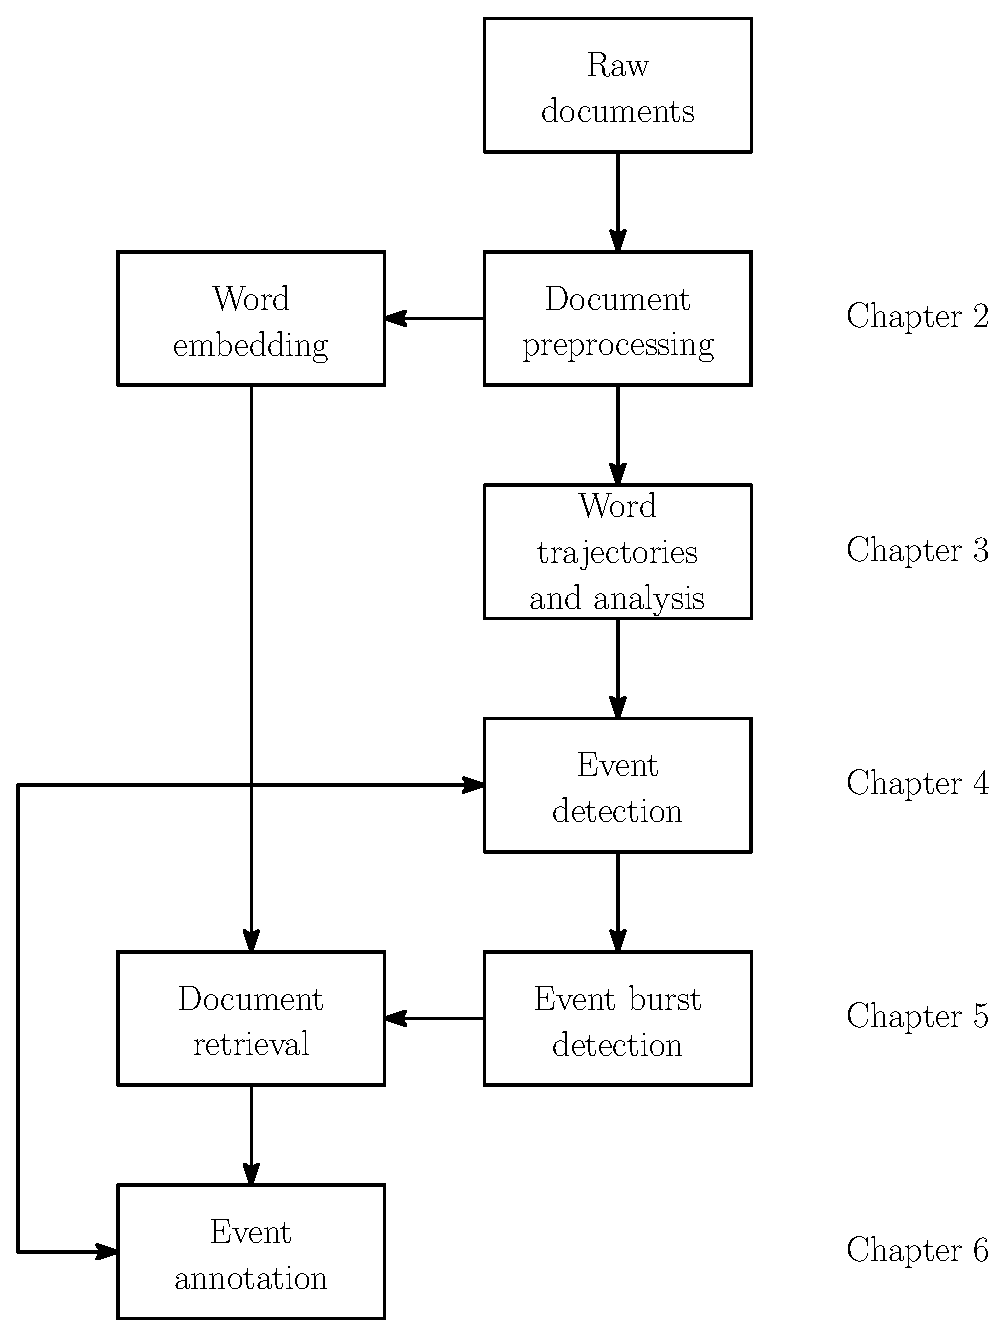
\includegraphics[height=0.6\paperheight]{diagram}
  \caption{Schematic representation of our method.}
  \label{fig:diagram}
\end{figure}

\chapter{Event detection algorithm}
%\begin{figure}[h]
%    \centering
%	\includegraphics[scale=0.5]{graph}
%	\caption{An example graph}
%	\label{fig:x sine graph}
%\end{figure}


\newcommand{\doccount}{N}
\newcommand{\featcount}{V}
\newcommand{\streamlen}{T}
\newcommand{\traj}{y}
\newcommand{\df}{DF}
\newcommand{\featset}{\text{M}}
\newcommand{\cost}{\text{C}}

\newcommand{\docoverlap}{\text{d}}
\newcommand{\featsim}{\text{JSD}}

\newcommand{\bowmat}{\mat{B}}
\newcommand{\dtdmat}{\mat{D}}
\newcommand{\trajmat}{\mat{T}}


The core of this algorithm is taken from \cite{event-detection}.

\section{Document fetching}
We assume a collection of $N$ documents $\left\{ d_{1}, d_{2}, \dots, d_{\doccount} \right\}$ where for each document $d_{i}$, its publication day $t_{i}$ is known. Then, the documents can be understood as a stream $\left\{ (d_{1}, t_{1}), (d_{2}, t_{2}), \dots, (d_{\doccount}, t_{\doccount}) \right\}$ with $t_{i} \leq t_{j}$ for $i < j$. Furthermore, we define $\streamlen$ to be the length of the stream, and we normalize the document publication days to be relative to the document stream start; that is $t_{1} = 1$ and $t_{\doccount} = \streamlen$.


\section{Binary bag of words model}
% TODO: blah blah we use the well known (binary) bag of words model, which drops the word order
To vectorize the documents, we define a matrix $\bowmat \in \left\{ 0, 1 \right\}^{\doccount \times \featcount}$, where $\featcount$ is the total vocabulary size. The document collection can then be interpreted as a set of $\doccount$ observations, each consisting of $\featcount$ binary features. The matrix $\bowmat$ is defined as

\begin{equation} \label{eq:bow-matrix}
	\bowmat_{ij} \coloneqq
	\begin{cases}
		1, & \text{document}~i~\text{contains the feature}~j \text{;} \\
		0, & \text{otherwise.}
	\end{cases}
\end{equation}

To limit the feature space, we trim the words appearing in less than 30 documents or in more than 90\% of the documents. The idea behind this is that the words appearing only in few documents cannot possibly represent relevant events, and are mostly anomalies. On the other hand, words appearing in most of the documents are likely stopwords, and do not carry much information. This helps to prune the feature space and makes $\bowmat$ reasonably sized.

From now on, we focus our analysis on the individual word features rather than whole documents.


\section{Computing feature trajectories}
The previous section represented word features in the document domain. This section focuses on representing these features in the time domain.

The time trajectory of a feature $f$ is a vector $\vect{\traj}_f = \left[ \traj_{f}(1), \traj_{f}(2), \dots, \traj_{f}(\streamlen) \right]$. Each element $\traj_{f}(t)$ represents the relative frequency of the feature $f$ at time $t$. This frequency is defined using the DFIDF score:

\begin{equation}
	\traj_{f}(t) \coloneqq \underbrace{\frac{\text{\df}_{f}(t)}{\text{\doccount}(t)}}_{\text{DF}} \times \underbrace{\log{\frac{\doccount}{\text{\df}_{f}}}}_{\text{IDF}},
\end{equation}

where $\text{\df}_{f}(t)$ is the number of documents published on day $t$ containing the feature $f$ (time-local document frequency), $\text{\doccount}(t)$ is the number of documents published on day $t$ and $\text{\df}_{f}$ is the number of documents containing the feature $f$ (global document frequency).

These feature trajectories are stored in a matrix $\trajmat \in \R^{\featcount \times \streamlen}$, with $\vect{\traj}_f$ being the $f$-th row of $\trajmat$. Here we take advantage of the normalization of the publication days, since they can now be used as column indices of $\trajmat$.

To make the computation efficient, we vectorize most of the operations. Along with the matrix $\bowmat$ defined in \ref{eq:bow-matrix}, we define a matrix $\dtdmat \in \left\{ 0, 1 \right\}^{\doccount \times \streamlen}$ mapping the documents to their publication days:

\begin{equation}
	\dtdmat_{ij} \coloneqq
	\begin{cases}
		1, & \text{document}~i~\text{was published on day}~j \text{;} \\
		0, & \text{otherwise}.
	\end{cases}
\end{equation}

Next, we sum the rows of $\bowmat$ together to obtain $\vect{\df} = \left[ \text{\df}_{1}, \text{\df}_{2}, \dots, \text{\df}_{\featcount} \right]$, and similarly the rows of $\dtdmat$ to obtain $\vect{\doccount}_{t} = \left[ \text{\doccount}(1), \text{\doccount}(2), \dots, \text{\doccount}(\streamlen) \right]$.

Using these matrices and vectors, we can compute $\trajmat$ as follows:

\begin{equation}
	\trajmat \coloneqq
		\underbrace{\text{diag} \left( \log{\frac{\doccount}{\vect{\df}}} \right)}_{\text{IDF}}
		\times
		\underbrace{\bowmat^{\T}
		\times \dtdmat
		\times \text{diag} \left( \frac{1}{\vect{\doccount}_{t}} \right)}_{\text{DF}}
\end{equation}


\section{Spectral analysis}
The next step is to employ spectral analysis techniques to discover periodicities in the features. Results from this section are further used to categorize the word features by their periodicity and signal power.

We apply the discrete Fourier transform to each feature trajectory, which represents the time series as a linear combination of $\streamlen$ complex sinusoids. We obtain $\mathcal{F} \vect{\traj}_{f} = \left[ X_{1}, X_{2}, \dots, X_{\streamlen}\right ]$ such that

\begin{equation*}
	X_{k} = \sum_{t = 1}^{\streamlen}{\traj_{f}(t) \me^{- \frac{2 \pi \mi}{\streamlen} (k - 1) t}}, ~ k = 1, 2, \dots, \streamlen.
\end{equation*}

The absolute value of the Fourier coefficient $X_{k}$ denotes the amplitude of the complex sinusoid at frequency $\frac{k}{\streamlen}$.

Having moved from the time domain to the frequency domain, we can now analyze the signal power and dominant periodicity of each feature.

We observe peaks in the power spectrum of the transformed data and obtain the signal power and periodicity from those. The power spectrum is estimated using the periodogram estimator

\begin{equation*}
	\vect{P} = \left[ \|X_{1}\|^{2}, \|X_{2}\|^{2}, \dots, \|X_{\ceil{\streamlen / 2}}\|^{2} \right].
\end{equation*}

To measure the overall signal power, we define the dominant power spectrum of the feature $f$ as the value of the highest peak in the power spectrum, that is

\begin{equation}
	\text{DPS}_{f} \coloneqq \max\limits_{k \leq \ceil{\streamlen / 2}}{\|X_{k}\|^{2}}.
\end{equation}

The dominant period is then defined as the inverse of the frequency corresponding to the highest peak:

\begin{equation}
	\text{DP}_{f} \coloneqq \frac{\streamlen}{\argmax\limits_{k \leq \ceil{\streamlen / 2}}{\|X_{k}\|^{2}}},
\end{equation}

When applied to rows of the matrix $\trajmat$, this method yields two vectors, $\vect{DPS} \in \R^{\featcount}$ and $\vect{DP} \in \R^{\featcount}$, containing the dominant power spectra and dominant periods, respectively.


\section{Feature categorization}
Based on the dominant power spectra and dominant periods, we divide the features into \underline{H}igh power-\underline{H}igh period and \underline{H}igh power-\underline{L}ow period categories \footnote{\cite{event-detection} actually define \textit{five} such categories; however, our method uses only the two sets of the most powerful features.}:

\begin{equation}
\begin{split}
	\text{HH} \coloneqq \left\{ f \mid \text{DPS}_{f} > \textit{dps-bound}, \text{DP}_{f} > \ceil{\streamlen / 2} \right\}, \\
	\text{HL} \coloneqq \left\{ f \mid \text{DPS}_{f} > \textit{dps-bound}, \text{DP}_{f} \leq \ceil{\streamlen / 2} \right\}.
\end{split}
\end{equation}

{\color{red}TODO: Define dps-bound!}


\section{Trajectory preprocessing}
During the event detection itself, we will need to measure the similarity of two trajectories. However, due to the general noisiness of the data, the similarities are not computed directly. Most features would then seem distant due to mild bursts malforming the trajectories, while not really contributing to the underlying events. Thus, the trajectories are first preprocessed.

\subsection{Burst filtering}
As we are only interested in the dominant bursts around the main events, we filter out the mild ones. We do this by computing a cutoff value for each feature trajectory and discarding all trajectory elements falling under this cutoff. This procedure is adopted from \cite{online-search-queries}. The algorithm is as follows:

\begin{algorithm}[H]
\begin{algorithmic}[1]
\caption{Burst filtering}
\Input $\text{window-length} ~ w$

\ForEach {$\vect{\traj}_{f} \in \{ \vect{\traj}_{1}, \vect{\traj}_{2}, \dots, \vect{\traj}_{\featcount}\}$}
	\State $\vect{MA}_{w} = \text{Moving Average of length} ~ w ~ \text{for} ~ \vect{\traj}_{f} = \left[ \traj_{f}(1), \traj_{f}(2), \dots, \traj_{f}(\streamlen) \right]$

	\State $\mathit{cutoff} = \text{mean} \left( \vect{MA}_{w} \right) + \text{std} \left( \vect{MA}_{w} \right)$

	\State $\vect{bursts}_{f} = \left[ \traj_{f}(t) \mid \traj_{f}(t) > \mathit{cutoff}, \traj_{f}(t) \in \vect{y}_{f} \right]$
\EndFor

\Output $\{ \vect{bursts}_{1}, \vect{bursts}_{2}, \dots, \vect{bursts}_{\featcount} \}$
\end{algorithmic}
\end{algorithm}

{\color{red} TODO: In the paper, they use $\vect{MA}(t)_{w} > \mathit{cutoff}$, try that. Also, why did I miss that? :(}

\subsection{Normalization}
From now on, we assume the individual trajectories have been normalized to have unit sums. This can be computed efficiently by vectorizing the operation and dividing every row of $\trajmat$ by its sum. Thanks to this normalization, the individual trajectories can be interpreted as probability distributions over the stream days.

\subsection{Smoothing}

We smoothen each trajectory by fitting a probability density function to it. Preserving the probability interpretation allows us to measure trajectory distance using information divergence later. Different techniques must be employed when smoothing aperiodic and periodic feature trajectories, since we aim mainly to fit all non-trivial bursts.

In this section, we interpret the trajectories as two-dimensional observations $\traj_{f} = \{ \left( 1, \traj \left(1 \right) \right), \left( 2, \traj \left(2 \right) \right), \dots, \left( \streamlen, \traj \left(\streamlen \right) \right) \}$.

\begin{enumerate}

\item \textbf{Aperiodic features}

An aperiodic feature trajectory $\traj_{f}$ is modeled by a Gaussian distribution. We fit the Gaussian function

\begin{equation*}
	f(x) = \frac{1}{\sigma \sqrt{2 \pi}} \me^{-\frac{\left( x - \mu \right)^{2}}{2 \sigma^{2}}}
\end{equation*}

to the trajectory $y_{f}$. The parameters $\mu$ and $\sigma$ are estimated using non-linear Least squares method. Unlike \cite{event-detection} who use the EM algorithm, Least squares proved to be less prone to outliers, yielding a shape more resembling the actual trajectory.

\item \textbf{Periodic features}

A periodic feature trajectory $\traj_{f}$ is modeled using a mixture of $K = \floor{\streamlen / \text{DP}_{f}}$ Cauchy distributions:

\begin{equation*}
	f(x) = \sum_{k = 1}^{K}{\alpha_{k} \frac{1}{\pi \gamma_{k} \left( 1 + \left( \frac{x - \mu_{k}}{\gamma_{k}} \right)^2 \right)}}
\end{equation*}

The mixing parameters $\alpha_{k}, \sum_{k = 1}^{K}{\alpha_{k}} = 1$, location parameters $\mu_{k}$ and scale parameters $\gamma_{k}$ are estimated using the EM algorithm.

The Cauchy distribution has a narrower peak and thicker tails than the Gaussian distribution, which models the periodic bursts more closely. The individual bursts of a periodic feature tend to be quite short, but even between two consecutive bursts, the frequency remains at a non-negligible level, which makes the Cauchy distribution a somewhat better choice.

\end{enumerate}


\section{Event detection}

During the event detection phase, the aim is to find sets of word features highly correlated both in the time domain and in the document domain. The assumption is that words appearing in similar documents during the same time period concern the same real-world events. Each such feature set then represents a single event.

By inspecting only the high power features, we uncover only the features best describing the individual events. This also helps to reduce computation time, since there are generally much fewer high power features than the low power ones.

The aperiodic and periodic features are detected separately, since we assume no connection between aperiodic events and the periodic ones.


\subsection{Measuring trajectory similarity}

Similarity between two feature trajectories is defined in terms of their information divergence. Unlike \cite{event-detection}, we use the \textit{Jensen-Shannon} divergence:

\begin{equation*}
	\featsim \left( \vect{p} \| \vect{q} \right) = \frac{1}{2} \text{D} \left( \vect{p} \| \vect{m} \right) + \frac{1}{2} \text{D} \left( \vect{q} \| \vect{m} \right),
\end{equation*}

where $\vect{m} = \frac{1}{2} \left( \vect{p} + \vect{q} \right)$ and D denotes the \textit{Kullback-Leibler} divergence.

The JS-divergence is symmetric, and its square root is a proper metric. It can also be computed without using the \textit{max} function, as opposed to the original approach, which makes the computation somewhat faster.

This similarity is then generalized to a set of features $\featset$ as

\begin{equation}
	\featsim \left( \featset \right) = \max{ \{ \featsim ( \vect{y}_{f_{i}} \| \vect{y}_{f_{j}} ) \mid f_{i}, f_{j} \in \featset \} }
\end{equation}


\subsection{Measuring document overlap}

The document overlap is first defined for two features, and then generalized to a whole feature set.

Let $\featset_{i}$ be the set of all documents containing a feature $f_{i}$, and $\featset_{j}$ the set of all documents containing a feature $f_{j}$. Then, the document overlap of the features $f_{i}$ and $f_{j}$ is defined as

\begin{equation}
	\docoverlap(f_{i}, f_{j}) \coloneqq \frac{\left\vert{\featset_{i} \cap \featset_{j}}\right\vert}{\min \left( {\left\vert{\featset_{i}}\right\vert, \left\vert{\featset_{j}}\right\vert} \right)}.
\end{equation}

Using this definition, the document overlap of a set of features $\featset$ can be defined as

\begin{equation}
	\docoverlap \left( \featset \right) \coloneqq \min{\{ \docoverlap \left( f_{i}, f_{j} \right) \mid f_{i}, f_{j} \in \featset \}}.
\end{equation}

Since we aim to maximize the document overlap among a set of features, it makes sense to define it using minimum, as it takes care of the worst possible case.


\subsection{Event detection}

We can now measure the similarity of a feature set both in the time domain (using JS-divergence) and in the document domain (using document overlap). These two measures are combined into a cost function $\cost$, which we aim to minimize.

\begin{equation} \label{eq:cost-function}
	\cost \left( \featset \right) \coloneqq \frac{\featsim \left( \featset \right)}{\docoverlap \left( \featset \right) \sum_{f \in \featset}{\text{DPS}_{f}}}
\end{equation}

Intuitively, a set $\featset$ which minimizes this function will have low inter-feature divergence, high document overlap and will be comprised of relevant features with high DPS.

To perform the event detection itself, we mostly adapt the \textit{Unsupervised greedy event detection} algorithm from \cite{event-detection}.

\begin{algorithm}[H]
\begin{algorithmic}[1]
\caption{Unsupervised greedy event detection}
\Input $\text{Feature set} ~ \featset \coloneqq \text{HH or HL}$

\State $\text{Sort the features in ascending DPS order: } DPS_{f_{1}} \leq DPS_{f_{2}} \leq \dots \leq DPS_{f_{\left\vert M \right\vert}}$

\State $k = 0$

\ForEach{$f \in \featset$}
	\State $k = k + 1$	
	\State $e_{k} = \{ f \}$
	\State $\cost \left(e_{k} \right) = \frac{1}{DPS_{f}}$
	\State $\featset = \featset \setminus f$
	
	\While{$M \neq \emptyset$}
		\State $m = \argmin\limits_{m}{\cost \left( e_{k} \cup f_{m} \right)}$

		\If{$\cost \left( e_{k} \cup f_{m} \right) < \cost \left( e_{k} \right)$}
			\State $e_{k} = e_{k} \cup f_{m}$
			\State $\featset = \featset \setminus f_{m}$
		\Else
			\Break
		\EndIf
	\EndWhile
\EndFor

\Output $\{ e_{1}, e_{2}, \dots, e_{k} \}$
\end{algorithmic}
\end{algorithm}

We do make two changes, however. First, we sort the features in \textit{ascending} rather than descending order. This ensures that words with lower DPS value will get selected first and that the function \ref{eq:cost-function} will not be minimalized as quickly. As a result, the events will contain more representing features and will not be broken into several events concerning the same real-world event. This effectively relaxes the DPS part of the function \ref{eq:cost-function} while keeping emphasis on the trajectory similarity and document overlap.

Second, we output the events as sets of word features rather than event trajectories. This is simply because we will need to access the individual features, and later, documents, of each event.

Note that due to the usage of set intersection in the document overlap definition, every event will be comprised of words appearing in exactly the same documents. This makes it trivial to retrieve the documents later, but tends to select a relatively low number of features for each event.

{\color{red} TODO: quote this: https://arxiv.org/pdf/1109.2378v1.pdf, the original article of the used method and the information retrieval book when writing about agglomerative clustering, use cosine similarity, compute test statistics from scipy to determine the method to use, also quote the article with Cauchy distribution}

\chapter*{Conclusion}
\addcontentsline{toc}{chapter}{Conclusion}
We examined how event detection methods depending on keyword representation could be improved by considering word embedding models, namely the Word2Vec model \citep{word2vec}. We tried to augment an existing method by \cite{event-detection} to use a Word2Vec-based similarity function to match semantically related words together. This did not bring significant improvement -- although the detected events were richer and less redundant, a notable amount of noise appeared. This made the events hard to assign to their real world counterparts, as most of their keywords did not contribute to any underlying topic.

Then, we explored a different approach, where we interpreted the keyword-based event detection as a literal clustering task. We defined a custom distance function also utilizing the Word2Vec model as a semantic measure. We then applied a clustering algorithm equipped with this distance function to words previously selected as eventful. Our evaluation suggests that this method was more successful than both the original method and its Word2Vec modification. The resulting events were composed mostly of representative words and reached lesser redundancy and noisiness than the previous methods.

The disadvantage of both our methods is the necessity to train the Word2Vec model, which is time consuming. However, it can be trained once and than reused for subsequent detections, as long as the document vocabulary remains similar.

We also examined how the Word2Vec model could be used to retrieve documents concerning the detected events. We applied the Word Mover's Distance \citep{wmd} to documents within each event's bursty period as a measure of their relevance to that particular event's keyword set. We then selected the most relevant documents as the event's document representation. Although the documents were of high quality and represented the events well, the process took an unbearable amount of time. In the original method, the retrieval process was more straightforward and much more efficient.

Finally, we applied multi-document summarization techniques to the documents to obtain a short summary describing each event. This, along with the event's occurrence dates and document sets, are the outputs of our method presented to the user. The summaries serve the purpose of giving a quick reference of the event's topic, based on which the user may decide to examine the event further and go through the retrieved documents.

In future work, it would be beneficial to use a more efficient way of computing the documents relevant to each event. Traditional information retrieval techniques, such as Latent Semantic Indexing \citep{lsi} could be used here, perhaps with some domain specific knowledge of the underlying events, such as their bursty periods.

Also, we would like to examine how an event could be represented directly as a set of documents, rather than words. Although there are attempts to do so \citep{document-bursty-representation}, they require to fine-tune a number of parameters, and the document representation is again constructed using word trajectories. The Doc2Vec model \citep{doc2vec}, a generalization of Word2Vec able to embed whole documents in a vector space, could be used to obtain the semantic representation.

Instead of computing a cutoff value to clean a word or an event trajectory, as we did in \autoref{chap:event-detection}, further signal processing techniques could be applied on the trajectories to separate the dominant bursts from the underlying noise. The result would be a somewhat cleaner trajectory devoid of any milder bursts of no interest. This could lower the noisiness, since words would be matched together based on only the dominant activity, not any underlying influence, which still eludes the cutoff value method.


% Appendices
\appendix
\chapter{Appendix Title}
\input{tex/chapters/appendix}


% Bibliography
\printbibliography

\end{document}